% \listfiles
\documentclass{beamer}
\mode<presentation>
\usecolortheme{crane}

\hfuzz=20pt
\setlength{\tabcolsep}{9pt}
\renewcommand{\arraystretch}{1.5}

\setbeamertemplate{navigation symbols}{
\usebeamerfont{footline}
\usebeamercolor[fg]{footline}
\hspace{1em}
\insertframenumber/\inserttotalframenumber
}

\setbeamertemplate{caption}{\raggedright\insertcaption\par}


\usepackage{xifthen}
\usepackage{anyfontsize}
\usepackage{fontawesome}
\usepackage{filecontents}
\usepackage{bm}
\usepackage{tikz}
\usepackage{pgfplots}

\pgfplotsset{compat=1.15}
\usetikzlibrary{
	positioning
	,plotmarks
	,shapes.callouts	
    ,intersections	
	,decorations.pathreplacing
	,patterns
}
% Commands
\newcommand{\edge}[3][]{
	\draw[#1] (#2) edge (#3);
}

\newcommand{\edgeWithLabel}[4][]{
	\draw[#1] (#2) edge node[edge label]{#3} (#4);
}

\newcommand{\twocolors}[1]{
	\fill[fill=orange] (#1.west) -- (#1.east) arc(0:180:7.5pt);
	\fill[fill=blue] (#1.west) -- (#1.east) arc(0:-180:7.5pt);
	\node at(#1){};
}

% Animation
\tikzset{
	on/.code args={<#1>#2}{
  		\only<#1>{\pgfkeysalso{#2}}
	},
	alt/.code args={<#1>#2#3}{
  		\alt<#1>{\pgfkeysalso{#2}}{\pgfkeysalso{#3}}
	},
	hide/.style={
		opacity=0
	},
	show/.style={
		opacity=1
	},
	hide nodes/.style={
		every node/.append style={hide}
	},
	hide nodes text/.style={
		every node/.append style={text=white}
	},
	show nodes/.style={
		every node/.append style={show}
	},
	show nodes text/.style={
		every node/.append style={text=black}
	},
	blur/.style={
		opacity=0.2
		,text=white
	}
}

% Note
\tikzset{
	note/.style={
		rectangle callout
		,fill=#1
		,thin
		,inner sep=1mm
	}
	,noteorange/.style={note=orange!50}
}


% Label
\tikzset{
	label/.style={
		rectangle,	
		draw=none,
		fill=white,
		% font=\tiny,
		% font=\scriptsize,
		font=\footnotesize,
		inner sep=2pt,
		minimum height=0,
		minimum width=0,
	},
	edge label/.style={
		label,
		midway,
		sloped,
	},
	edge label below/.style={edge label, below=1mm},
	edge label above/.style={edge label, above=1mm},
}


% DEFAULTS
\tikzset{default node/.style={
	draw, 
	circle,
	inner sep=0mm,
	minimum size=5mm,
	font=\small,
}}

\tikzset{
	>=latex
	,every node/.style={default node}
	,every picture/.append style={very thick, black!70}
}
\newtheorem{observation}{Observation}

\DeclareMathOperator*{\argmin}{arg\,min}
\DeclareMathOperator*{\argmax}{arg\,max}

\def\R{\mathbb{R}}
\def\N{\mathbb{N}}

\def\1star{{\color{orange} \faStar}}
\def\2star{{\color{orange} \faStar\faStar}}
\def\3star{{\color{orange} \faStar\faStar\faStar}}

\def\pointer{callout absolute pointer}

\title{
Approximation Algorithms 
\\
for the
\\
Maximum Carpool Matching Problem
\\
and 
\\
Submodular Maximization
}
\author[shortname]{
    \textbf{Gilad Kutiel}
}
\date{2019}


\begin{document}

\begin{frame}
\titlepage
\end{frame}


\begin{frame}{Combinatorial Optimization}
\Huge Finding an \textbf{optimal object} from a \textbf{finite set} of objects.
\end{frame}
\begin{frame}{Example - MST}
    \begin{center}
        \begin{tikzpicture}[x=1.5cm,y=1.5cm]

	\foreach[count=\i] \a \r in{
		0/1
		,10/2
		,30/3
		,160/1
		,230/1
		,-40/2
		,100/1
		,80/2
		,-10/3
		,20/4
		,-100/2
		,-30/4
	}{
		\node(\i) at(\a:\r) {\i};
	}

	\foreach \u \w \v in{
		1/2/2%
		,1/2/4%
		,1/2/5%
		,1/3/6%
		,1/2/7%
		% 
		,2/1/3%
		,2/1/9%
		,2/1/10%
		% 
		,6/1/11%
		,6/3/12%
		% 
		,7/1/8%
	}{
		\edgeWithLabel[on=<2>{orange}]{\u}{\w}{\v}
	}

	\foreach \u \w \v in{
		% 
		% 
		3/1/10%
		% 
		,4/1/5%
		,4/1/7%
		% 
		,5/1/11%
		% 
		,6/1/9%
		% 
		% 
		,8/1/3%
	}{
		\edgeWithLabel[on=<2>{blur}]{\u}{\w}{\v}
	}

\end{tikzpicture}
    \end{center}
\end{frame}
\begin{frame}{Example - Star Forest}
    \begin{center}
        \begin{tikzpicture}[]
	\graph[
		random seed=2
		,spring layout
		,node distance=2cm
		,edge quotes={edge label}
	]{
		1,2,3,4,5,6,7,8,9,10,11,12;
		
		{[edges={on=<2>{blur}}]
		1 --["2"] 2;
		1 --["1"] 4;
		% 
		2 --["3"] 5;
		2 --["1"] 7;
		% 
		3 --["1"] 8;
		% 
		4 --["2"] 11;
		% 
		% 
		% 
		7 --["1"] 9;
		7 --["1"] 12;
		% 
		8 --["1"] 10;
		% 
		};
		
		{[edges={on=<2>{orange}}]
		1 --["1"] 3;
		% 
		2 --["3"] 6;
		% 
		4 --["2"] 6;
		% 
		5 --["2"] 8;
		5 --["1"] 9;
		5 --["2"] 10;
		% 
		6 --["2"] 7;
		6 --["2"] 12;
		% 
		};
	};
\end{tikzpicture}
    \end{center}
\end{frame}
\begin{frame}{Combinatorial Optimization}
\begin{itemize}[<+->]
  \item Artificial Intelligence, Machine Learning, Image Processing...
  \item Most problems are NP-hard.
	\begin{itemize}[<+->]
	  \item Heuristics.
	  \item Special Cases.
	  \item Parameterized Complexity.
	  \item \textbf{Approximation Algorithms}.
		\begin{itemize}[<+->]
			\item $\alpha$-approximation.
		\end{itemize}
	\end{itemize}
\end{itemize}
\end{frame}
\begin{frame}{1/2-Approximation Maximum Star Forest}
    \begin{center}
        \begin{tikzpicture}[x=1.5cm,y=1.5cm]
            \foreach[count=\i] \a \r in{
                0/1,10/2,30/3,160/1,230/1,-40/2,100/1,80/2,-10/3,20/4,-100/2,-30/4
            }{
                \node(\i) at(\a:\r) {};
            }
        
            \begin{scope}[on=<2>{orange}]
                \foreach \u \v in{
                    1/2,1/4,1/5,1/7%
                    ,6/12%
                }{
                    \edge[on=<3>{red}]{\u}{\v}
                }
                \foreach \u \v in{
                    1/6%
                    ,2/3,2/9,2/10%
                    ,6/11%
                    ,7/8%
                }{
                    \edge[on=<3>{blue}]{\u}{\v}
                }
            \end{scope}
        
            \foreach \u \v in{
                3/10%
                ,4/5,4/7%
                ,5/11%
                ,6/9%
                ,8/3%
            }{
                \edge[on=<2->{blur}]{\u}{\v}
            }
        \end{tikzpicture}
    \end{center}
\end{frame}

\begin{frame}
\vfill
\begin{center}
\Huge Maximum Carpool Matching
\end{center}
\vfill
\end{frame}

\begin{frame}{Maximum Carpool Matching}
\begin{center}
    \begin{tikzpicture}[x=2cm,y=1.5cm, ->]
        \foreach[count=\i] \a \r \c \p in{
            0/1/\faCar/\faFemale
            ,10/2/\faBicycle/\faMale
            ,30/3/\faCab/\faChild
            ,160/1/\faMotorcycle/\faFemale
            ,230/1/\faTruck/\faMale
            ,-40/2/\faCar/\faFemale
            ,100/1/\faBicycle/\faMale
            ,80/2/\faCab/\faFemale
            ,-10/3/\faMotorcycle/\faBlind
            ,20/4/\faTruck/\faMale
            ,-100/2/\faCar/\faFemale
            ,-30/4/\faBicycle/\faMale
        }{
            \node[draw=none, inner sep=1mm](\i) at(\a:\r) {\c~\p};
        }
    
        \pause
        \foreach \u \w \v in{
            1/2/5%
            ,8/5/7%
            ,9/6/6%
            ,10/5/2%
            ,11/4/5%
            ,12/3/6%
        }{
            \edgeWithLabel[bend left, on=<3>{orange}]{\u}{\w}{\v}
        }
    
        \foreach \u \w \v in{
            1/2/2,1/2/4,1/3/6,1/2/7%
            ,2/4/3%
            ,3/6/10%
            ,4/7/7%
            ,5/3/4,5/9/11%
            ,6/1/9,6/5/11%
            ,7/4/1,7/3/8%
            ,8/5/3%
        }{
            \edgeWithLabel[bend left, on=<3>{blur}]{\u}{\w}{\v}
        }
    
    \end{tikzpicture}
\end{center}
\end{frame}
\begin{frame}{Maximum Carpool Matching cont.}
\begin{center}
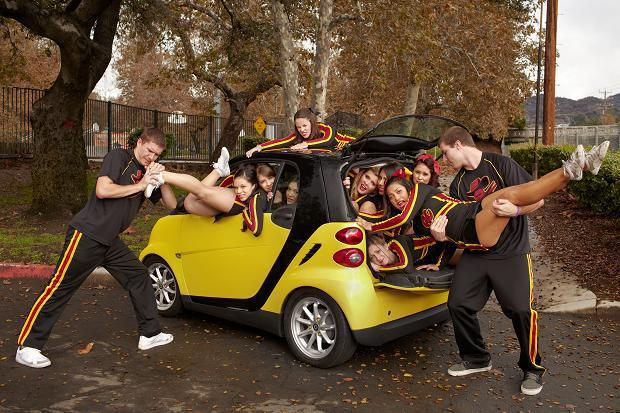
\includegraphics[scale=.5]{capacity}
\end{center}
\end{frame}
\begin{frame}{1/3 Approximation CP}
\begin{center}
\tikzset{
	col1/.style={orange}
	,col2/.style={blue}
	,col3/.style={red}
	,col4/.style={brown}
	,col5/.style={green}
}

\begin{tikzpicture}[very thick]
\foreach[count=\i] \x \y \c in {
	0/0/1
	,1/2/2
	,2/-1/3
	,3/1/2
	,4/-2/1
}{
	\node[col\i, on=<5->{black}](\i) at(\x,\y){{\onslide<-4>{\c}}};
}

\foreach \u \v in {
	1/2%
	,4/5%
}{
	\draw[on=<7->{blue}] (\u) to[bend left] (\v);
}

\foreach \u \v in {
	2/4%
	,3/4%
}{
	\draw[on=<7->{green}] (\u) to[bend left] (\v);
}

\foreach \u \v in {
	5/3%
}{
	\draw[on=<6->{orange}] (\u) to[bend left] (\v);
}


\foreach \u \v in {
	1/3%
	,2/1%
	,3/1,3/5%
	,4/2,4/3%
}{
	\draw[on=<4->{blur}] (\u) to[bend left] (\v);
}

\begin{scope}[xshift=6cm, yshift=-3cm, x=15mm]
\onslide<2-4>{
\foreach[count=\i] \c in {1,2,3,2,1}{
	\node[col\i](l\i) at(0,\i){1};
	\node[col\i](r\i) at(2,\i){\c};
}

\foreach \u \v in {
	1/2%
	,2/4%
	,3/4%
	,4/5%
	,5/3%
}{
	\draw[] (l\u) -- (r\v);
}

\foreach \u \v in {
	1/3%
	,2/1%
	,3/1,3/5%
	,4/2,4/3%
}{
	\draw[on=<3->{blur}] (l\u) -- (r\v);
}
}
\end{scope}

\end{tikzpicture}
\end{center}
\end{frame}

\begin{frame}
\vfill
\begin{center}
\Huge Submodular Functions
\end{center}
\vfill
\end{frame}

\begin{frame}{Submodular Functions}
\begin{align*}
    & f(A \cup B) + f(A \cap B) \leq f(A) + f(B)
    \\
    \\
    & \text{Or}
    \\
    \\
    \forall A \subseteq B \quad & f(A \cup \{x\}) - f(A) \geq f(B \cup \{x\}) - f(B)
    \\
\end{align*}
\end{frame}
\begin{frame}{Example - Cut}
\begin{center}
$f(A \cup B) + f(A \cap B) \leq f(A) + f(B)$
\end{center}
\begin{center}
\begin{tikzpicture}[]

    \node(1) at(0:2) {1};
    \node[fill=orange](2) at(120:2) {2};
    \node[fill=blue](3) at(240:2) {3};

    \twocolors{1}

    \draw[on=<3>{blue}] (1) -- (2) coordinate[midway](12);
    \draw[on=<2>{orange},on=<3>{blue}] (2) -- (3);
    \draw[on=<2>{orange}] (3) -- (1) coordinate[midway](13);

    \onslide<4>{
        \draw[orange](1) -- (12);
        \draw[blue](12) -- (2);
        \draw[orange](1) -- (13);
        \draw[blue](13) -- (3);
    }
    \onslide<5>{
        
    }

\end{tikzpicture}
\end{center}
\end{frame}
\begin{frame}{Example - Coverage}
    \begin{center}
        $$f(A \cup B) + f(A \cap B) \leq f(A) + f(B)$$
        \begin{tikzpicture}[x=2cm]

            \begin{scope}[yshift=.5cm,every node/.append style={rectangle}]
                \node[fill=blue](l1) at(0,0){};
                \node[](l2) at(0,1){};
                \node[fill=orange](l3) at(0,2){};
            \end{scope}
            
            \fill[fill=blue] (l2.west) rectangle (l2.south east);
            \fill[fill=orange] (l2.west) rectangle (l2.north east);
            \node[rectangle] at(l2){};
        
            \node[on=<2>{fill=blue}](r1) at(2,0){};
            \node[on=<2>{fill=blue},on=<3>{fill=orange}](r2) at(2,1){};
            \node[on=<2>{fill=blue},on=<3>{fill=orange}](r3) at(2,2){};
            \node[on=<3>{fill=orange}](r4) at(2,3){};
        
            \onslide<4>{
                \twocolors{r2}
            }
        
            \onslide<5>{
                \twocolors{r1}
                \twocolors{r2}
                \twocolors{r3}
                \twocolors{r4}
            }
        
            \foreach \l \r in{
                1/1,1/3%
                ,2/2%
                ,3/3,3/4%
            }{
                \edge{l\l}{r\r};
            }
        
        \end{tikzpicture}
    \end{center}
\end{frame}

\begin{frame}
\vfill
\begin{center}
\Huge 
Budgeted Maximum Coverage
\end{center}
\vfill
\end{frame}

\begin{frame}{Budgeted Maximum Coverege}
    \begin{center}
        $$
        \beta = 2
        $$
        \begin{tikzpicture}[x=2cm]

    \tikzset{
        sel/.style={fill=green}
        ,drop/.style={fill=red}
    }
    \begin{scope}[yshift=.5cm,every node/.append style={rectangle}]
        \node[on=<3->{sel}](l1) at(0,0){1};
        \node[on=<2->{sel}](l2) at(0,1){1};
        \node[on=<4->{drop}](l3) at(0,2){3};
        \node[on=<5->{sel}](l4) at(0,3){1};
        \node[on=<6->{drop}](l5) at(0,4){2};
    \end{scope}
    
    \node[on=<3->{sel}](r1) at(2,0){3};
    \node[on=<2->{sel}](r2) at(2,1){2};
    \node[on=<2->{sel}](r3) at(2,2){4};
    \node[](r4) at(2,3){5};
    \node[on=<5->{sel}](r5) at(2,4){2};
    \node[](r6) at(2,5){1};

    \foreach \l \r in{
        1/1,1/2%
        ,2/2,2/3%
        ,3/3,3/4,3/5%
        ,4/5%
        ,5/5,5/6%
    }{
        \edge{l\l}{r\r};
    }

\end{tikzpicture}
    \end{center}
\end{frame}
\begin{frame}{Greedy - Bad}
    \begin{center}
        
        $$\beta = k$$
        \begin{tikzpicture}[x=2cm]
        \begin{scope}[every node/.append style={rectangle}]
            \node[](l1) at(0,1){1};
            \node[](l2) at(0,2){k};
        \end{scope}
        
        \node[](r1) at(2,1){2};
        \node[](r2) at(2,2){k};
        
        \foreach \l \r in{
            1/1,2/2%
        }{
            \edge{l\l}{r\r};
        }
                
        \end{tikzpicture}
    \end{center}
\end{frame}
\begin{frame}{Greedy - Lemma}
    \begin{lemma}
        $$f(G) \geq (1 - e^{-\frac{|G|}{|O|}})f(O)$$
    \end{lemma}
    \pause
    \begin{center}
        $$\beta = 4$$
        \begin{tikzpicture}[x=2cm]
            \tikzset{
                sel/.style={fill=green}
                ,drop/.style={fill=red}
            }
            \begin{scope}[yshift=.5cm,every node/.append style={rectangle}]
                \node[on=<3->{sel}](l1) at(0,0){1};
                \node[on=<2->{sel}](l2) at(0,1){1};
                \node[](l3) at(0,2){3};
            \end{scope}
            
            \node[on=<3->{sel}](r1) at(2,0){2};
            \node[on=<2->{sel}](r2) at(2,1){3};
            \node[](r3) at(2,2){2};
            \node[](r4) at(2,3){2};
        
            \foreach \l \r in{
                1/1%
                ,2/2%
                ,3/2,3/3,3/4%
            }{
                \edge{l\l}{r\r};
            }
            \onslide<4>{
                \draw[decorate,decoration={brace,amplitude=10pt}]
                ([xshift=-2mm]l1.south west) -- ([xshift=-2mm]l2.north west)
                node[midway, draw=none, left=5mm]{$\geq (1 - e^{-\frac{1}{2}})f(O)$};
            }
        \end{tikzpicture}    
    \end{center}
\end{frame}

\begin{frame}{Modified Greedy}
    \begin{center}
        $$\beta = 4$$
        \begin{tikzpicture}[x=2cm]
            \tikzset{
                sel/.style={fill=green}
                ,drop/.style={fill=red}
            }
            \begin{scope}[yshift=.5cm,every node/.append style={rectangle}]
                \node[on=<3>{sel}](l1) at(0,0){1};
                \node[on=<2-3>{sel}](l2) at(0,1){1};
                \node[on=<5>{sel}](l3) at(0,2){3};
            \end{scope}
            
            \node[on=<3>{sel}](r1) at(2,0){2};
            \node[on=<{2-3,5}>{sel}](r2) at(2,1){3};
            \node[on=<5>{sel}](r3) at(2,2){2};
            \node[on=<5>{sel}](r4) at(2,3){2};
        
            \foreach \l \r in{
                1/1%
                ,2/2%
                ,3/2,3/3,3/4%
            }{
                \edge{l\l}{r\r};
            }
        \end{tikzpicture}    
    \end{center}
\end{frame}
\begin{frame}{Submodular - Previous Result}
    \begin{center}
        \Large
        \begin{tabular}{l l l}
            \hline
            $O(n^2)$
            &
            $1 - e^{-\frac{1}{2}}$
            &
            $\approx 0.39$
            \\
            \color{orange}$O(n^2)$
            &
            \color{orange}$1 - e^{-(\frac{1}{2} + 0.104)}$
            &
            $\approx 0.45$
            \\
            \color{orange}$O(n^2)$
            & 
            \color{orange}$1 - e^{-\frac{2}{3}}$ 
            &
            $\approx 0.49$
            \\
            $O(n^5)$
            & 
            $1 - e^{-1}$ 
            &
            $\approx 0.63$
            \\
            $\frac{1}{\epsilon}^{O(\epsilon^{-4})}n \log^2 n$
            & 
            $1 - e^{-1} - \epsilon$ 
            &
            $\approx 0.63 - \epsilon$
            \\
            \hline
        \end{tabular}
        
    \end{center}
\end{frame}
% 
\begin{frame}{Bucket Algorithm}
\begin{center}
\begin{tikzpicture}[every node/.style={}]
\begin{axis}[
    axis lines=left
    ,ticks=none
    ,ymin=0
    ,ymax=10
    ,xmin=0
    ,xmax=10
    ,xlabel={Cost}
    ,ylabel={Profit}
    ]
    \addplot[
        ,only marks
        ,every mark/.style={draw=white, fill=black}
    ] coordinates {
        (1,2) (1,4) 
        (2,3) (2,6)
        (3,5) (3,7)
        (4,3) (4,6) (4,8)
        (5,7) (5,8) (5,10)
        (6,2) (6,5) (6,7) (6,9)
        (7,3) (7,9)
        (8,5) (8,10)
        (9,2) (9,4) (9,7) (9,8)
    };
        
\end{axis}
\end{tikzpicture}
\end{center}
\end{frame}
\begin{frame}{Bucket Algorithm - Analysis}
    \def\pLarge{P_{\text{large}}}

    \begin{columns}
    
        \begin{column}{0.3\textwidth}
            \begin{itemize}[]
                \pause
                \item $\frac{f(\pLarge)}{f(O)} \approx 1 $ \pause \faThumbsOUp
                \pause
                \item $\frac{f(\pLarge)}{f(O)} \approx 0 $ \pause \faThumbsOUp
            \end{itemize}
        \end{column}

        \pause
        \begin{column}{0.6\textwidth}
            
            \begin{tikzpicture}[every node/.style={}]
                \begin{axis}[
                    ,width=.9\textwidth
                    ,domain=0:0.33
                    ,ymin=0
                    ,ymax=1
                    ,yticklabels={,,}
                    ,extra y ticks={
                        0.486582880967
                    }
                    ,extra y tick labels={
                        $1 - e^{-\frac{2}{3}}$
                    }
                    ,xmax=.34
                    ,ytick distance=2
                    ,xtick distance=.1
                    ,xlabel=$\delta$
                    ,axis lines=left
                ]
                    \addplot[very thin]{
                        0.486582880967
                    };

                    \addplot[orange]{
                        1 - exp(-(2/3 + x)/(1 - 1/3 - 1/3 + x))
                    };
                \end{axis}
            \end{tikzpicture}

        \end{column}

    \end{columns}
    \pause
    \begin{theorem}
        Bucket Algorithm is a $(1 - e^{-\frac{2}{3}})$-approximation algorithm.
    \end{theorem}

\end{frame}
\begin{frame}{Submodular - Conclusion}
    \begin{center}
        \Large
        \begin{tabular}{l l}
            \hline
            $1 - e^{-\frac{1}{2}}$ & $O(n^2)$
            \\
            \color{orange}$1 - e^{-\frac{2}{3}}$ & \color{orange}$O(n^2)$
            \\
            $1 - e^{-1}$ & $O(n^5)$
            \\
            $1 - e^{-1} - \epsilon$ & $\frac{1}{\epsilon}^{O(\epsilon^{-4})}n \log^2 n$
            \\
            \hline
        \end{tabular}
        
        \vfill
        
        \pause
        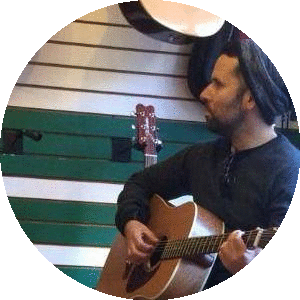
\includegraphics[height=2cm]{ariel.png}
        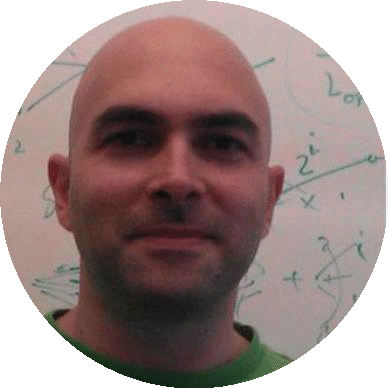
\includegraphics[height=2cm]{roy.png}
        
    \end{center}
\end{frame}

\begin{frame}
    \vfill
    \begin{center}
    \Huge 
    Maximum Carpool Matching
    \\
    (Revisited)
    \end{center}
    \vfill
\end{frame}
\begin{frame}{Maximum Carpool Matching}
    \begin{columns}
        \begin{column}{0.5\textwidth}
            \begin{tikzpicture}[every node/.style={draw=none,rectangle}, y=1.3cm]
                \foreach[count=\i] \a \r \c \p in{
                    0/0/\faCar/\faFemale
                    ,10/2/\faBicycle/\faMale
                    ,30/3/\faCab/\faChild
                    ,160/2/\faMotorcycle/\faFemale
                }{
                    \node[](p\i) at(\a:\r) {\c~\p};
                }
                
                \foreach[count=\i] \a \r \c \p in {
                    240/2/\faTruck/\faMale
                    ,-40/2/\faCar/\faFemale
                    ,100/2/\faBicycle/\faMale
                }{
                    \node[on=<2->{orange}](d\i) at(\a:\r) {\c~\p};
                }

                \foreach \u \v in{
                    p1/p2,p1/p4,p1/d1,p1/d2%
                    ,p2/p3,p2/d3%
                    ,p3/d3%
                    ,p4/d3,p4/d1%
                    ,d1/d2%
                }{
                    \draw (\u) -- (\v);
                }
            \end{tikzpicture}
        \end{column}
        \begin{column}{0.4\textwidth}
            \onslide<3>{
            \begin{tikzpicture}[every node/.style={draw=none,rectangle}, y=1.3cm]
                \foreach[count=\i] \c \p in{
                    \faCar/\faFemale
                    ,\faBicycle/\faMale
                    ,\faCab/\faChild
                    ,\faMotorcycle/\faFemale
                }{
                    \node[](p\i) at(0,\i) {\c~\p};
                }
                
                \foreach[count=\i] \c \p in {
                    \faTruck/\faMale
                    ,\faCar/\faFemale
                    ,\faBicycle/\faMale
                }{
                    \node[on=<2->{orange}](d\i) at([yshift=.5cm]3,\i) {\c~\p};
                }

                \foreach \u \v in{
                    p1/d1,p1/d2%
                    ,p2/d3%
                    ,p3/d3%
                    ,p4/d3,p4/d1%
                }{
                    \draw (\u) -- (\v);
                }
            \end{tikzpicture}
            }
        \end{column}
    \end{columns}
\end{frame}
\newcommand{\group}[3]{
    \draw[#3, -, name path=#1#2]
        (#1.west)
        to[out=90,in=90] (#2.east)
        to[out=-90,in=-90] (#1.west)
        ;
}

\begin{frame}{Maximum Carpool Matching cont.}
\begin{center}
    \begin{tikzpicture}[
        every node/.append style={
            draw=none
            ,font=\Large
        }
        , y=1.45cm
        , x=1.5cm
        , very thick
        ]
        
        \onslide<+->
        % GROUP 1 
        \node(11) at(0,1){\faFemale};
        \node(12) at(1,1){\faFemale};
        \node(13) at(2,1){\faFemale};
        
        \begin{scope}[every node/.append style={orange}]
        \node(14) at(0,0){\faFemale};
        \node(15) at(1,0){\faFemale};
        \node(16) at(2,0){\faFemale};
        \end{scope}
        
        \group{14}{15}{purple}
        \group{15}{16}{cyan}
        
        \draw[green] (11) -- (14);
        \draw (12) -- (15);
        \draw[orange] (13) -- (16);
        
        % GROUP 2 
        \begin{scope}[yshift=-4cm]
        \node(21) at(0,1){\faFemale};
        \node(22) at(1,1){\faFemale};
        \node(23) at(2,1){\faFemale};
        \node(24) at(0,0){\faFemale};
        
        \begin{scope}[every node/.append style={orange}]
        \node(25) at(1,0){\faFemale};
        \end{scope}
        
        \node(26) at(2,0){\faFemale};
        \end{scope}
        
        \group{24}{25}{purple,dotted,thin}
        \group{25}{26}{cyan,dotted,thin}
        
        \draw[cyan,-, name intersections={of=2425 and 2526}]
        (intersection-1)
        to [out=210,in=150,looseness=1.40] (intersection-2)
        ;
        
        \draw[purple,-, name intersections={of=2425 and 2526}]
        (intersection-1)
        to [out=-30,in=30,looseness=1.40] (intersection-2)
        ;
        
        \draw[] (21) -- (25);
        \draw[orange] (24) -- (25);
        \draw[green] (26) -- (25);
        
        % LABELS
        \begin{scope}[every node/.style={black, rectangle}]
        \node[above=0 of 12]{$F(A \cup B)$};
        \node[below=5mm of 25]{$F(A \cap B)$};
        \end{scope}
        
        
        \onslide<+->
        % GROUP 3 
        \begin{scope}[xshift=7cm]
        \node(41) at(0,1){\faFemale};
        \node(42) at(1,1){\faFemale};
        \node(43) at(2,1){\faFemale};
        
        \begin{scope}[every node/.append style={orange}]
        \node(44) at(0,0){\faFemale};
        \node(45) at(1,0){\faFemale};
        \end{scope}
        
        \node(46) at(2,0){\faFemale};
        \end{scope}
        
        \group{44}{45}{purple}
        
        % GROUP 4 
        \begin{scope}[xshift=7cm, yshift=-4cm]
        \node(31) at(0,1){\faFemale};
        \node(32) at(1,1){\faFemale};
        \node(33) at(2,1){\faFemale};
        
        \node(34) at(0,0){\faFemale};
        
        \begin{scope}[every node/.append style={orange}]
        \node(35) at(1,0){\faFemale};
        \node(36) at(2,0){\faFemale};
        \end{scope}
        
        \end{scope}
        
        \group{35}{36}{cyan}
        
        % LABELS
        \begin{scope}[every node/.style={black, rectangle}]
        \node[above=0 of 42]{$F(A)$};
        \node[below=5mm of 35]{$F(B)$};
        \end{scope}
        
        % ARCS
        \onslide<+->
        \draw[green] (41) -- (44);
        \draw[green] (46) -- (45);
        \onslide<+->
        \draw[orange] (34) -- (35);
        \draw[orange] (33) -- (36);
        \onslide<+->
        \draw (42) -- (45);
        \draw (31) -- (35);
        
    \end{tikzpicture}
\end{center}
\end{frame}
\begin{frame}{Submodular}
\begin{itemize}[<+->]
  \item Let $D = \{{\color{brown}\text{\faFemale}, \ldots, \text{\faFemale}}\} \subseteq V$
  \item Let $F(D) = OPT$ (w.r.t D)
\end{itemize}

\onslide<+->
\begin{theorem}
$F$ is submodular
\end{theorem}

\onslide<+->
\begin{corollary}
MCM is $1/2$-approximable
\end{corollary}



\end{frame}
\begin{frame}{Many Variants}
\def\pointer{callout absolute pointer}
\vfill
\begin{center}
\begin{tikzpicture}[every node/.style={note=orange!50}, x=16mm]
\draw (0,0) -- (6,0);
\node[\pointer={(0,0)}] at(0, 1) {SF};
\node[\pointer={(1,0)}] at(1, -1) {Node weighted SF};
\node[\pointer={(2,0)}] at(2, 1) {Edge weighted SF};
\node[\pointer={(3,0)}] at(3, -2) {Unweighted, O(1) capacity CM};
\node[\pointer={(4,0)}] at(4, 2) {Unweighted CM};
\node[\pointer={(5,0)}] at(5, -1) {CM};
\node[\pointer={(6,0)}] at(6, 1) {Group CM};
\end{tikzpicture}
\end{center}
\vfill
\end{frame}
\begin{frame}{Results}
\centering
\begin{tikzpicture}[y=50mm, x=8mm, every node/.style={draw=none}, -]


\foreach \x in {6,...,17}{
	\draw (\x, 1pt) -- (\x, -3pt) node[anchor=north]{\tiny \x};
	\draw[thin, gray!20] (\x, 0) -- (\x, 1.1);
}

\foreach \y in {0.25,.5,...,1}{
	\draw (6, \y) -- +(1pt, 0) -- +(-3pt, 0) node[anchor=east]{\tiny \y};
	\draw[thin, gray!20] (6, \y) -- (18, \y);
}

\draw (6,-5pt) -- (6,1.1) node[anchor=south]{Ratio};
\draw (5,0) -- (18,0) node[anchor=west]{Year};

\begin{filecontents}{data-upper.txt}
7   0.996153846
8   0.95
8.8 0.91
\end{filecontents}

\begin{filecontents}{data-unweight.txt}
7   0.6
8   0.71
9   0.804
\end{filecontents}

\begin{filecontents}{data-weight-vertex.txt}
8   0.64
\end{filecontents}

\begin{filecontents}{data-weight-edge.txt}
7   0.5
\end{filecontents}

\begin{filecontents}{data-unweight-cp.txt}
16   0.5
\end{filecontents}

\begin{filecontents}{data-cp.txt}
16   0.33
17   0.5
\end{filecontents}

\begin{filecontents}{data-fixed-cp.txt}
17   0.75
\end{filecontents}

\tikzset{upper/.style={mark=*, mark options={fill=red}}}
\tikzset{unweight/.style={mark=triangle*, mark options={fill=blue}}}
\tikzset{weight-vertex/.style={mark=square*, mark options={fill=cyan}}}
\tikzset{weight-edge/.style={mark=diamond*, mark options={fill=green}}}
\tikzset{unweight-cp/.style={mark=heart, mark options={fill=orange}}}
\tikzset{cp/.style={mark=pentagon*, mark options={fill=purple}}}
\tikzset{fixed-cp/.style={mark=otimes*, mark options={fill=magenta}}}

\draw plot[upper] file {data-upper.txt};
\draw plot[unweight] file {data-unweight.txt};
\draw plot[weight-vertex] file {data-weight-vertex.txt}; 
\draw plot[weight-edge] file {data-weight-edge.txt};
\draw plot[unweight-cp] file {data-unweight-cp.txt};
\draw plot[cp] file {data-cp.txt};
\draw plot[fixed-cp] file {data-fixed-cp.txt};

\begin{scope}[xshift=15mm, yshift=7mm]
\draw 
plot[upper] (10,1) -- +(-5pt,0) -- +(5pt,0) 
node[right]{\tiny Hardness};

\draw[yshift=-\baselineskip] 
plot[unweight] (10,1) -- +(-5pt,0) -- +(5pt,0) 
node[right]{\tiny Unweighted SF};

\draw[yshift=-2\baselineskip] 
plot[weight-vertex] (10,1) -- +(-5pt,0) -- +(5pt,0) 
node[right]{\tiny Vertex Weighted SF};

\draw[yshift=-3\baselineskip] 
plot[weight-edge] (10,1) -- +(-5pt,0) -- +(5pt,0) 
node[right]{\tiny Edge Weighted SF};

\draw[yshift=-4\baselineskip] 
plot[unweight-cp] (10,1) -- +(-5pt,0) -- +(5pt,0) 
node[right]{\tiny Unweighted CP};

\draw[yshift=-5\baselineskip] 
plot[cp] (10,1) -- +(-5pt,0) -- +(5pt,0) 
node[right]{\tiny CP};

\draw[yshift=-6\baselineskip] 
plot[cp] (10,1) -- +(-5pt,0) -- +(5pt,0) 
node[right]{\tiny Fixed CP};

\end{scope}
\end{tikzpicture}
\end{frame}

\begin{frame}

\vfill

\begin{center}
{\Huge Thank You.}
\vfill
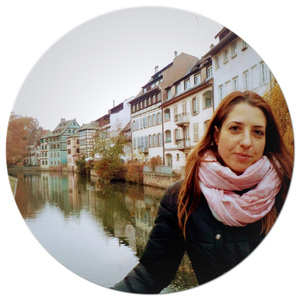
\includegraphics[height=2cm]{talia.png}
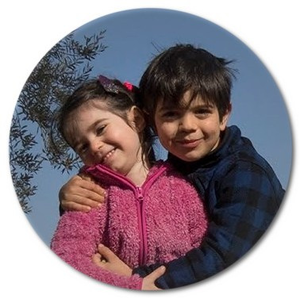
\includegraphics[height=2cm]{yoavyael.png}
\end{center}

\vfill


\end{frame}

\end{document}